\chapter{Examples}

\section{Figures}



\begin{figure} [H]
	\centering
	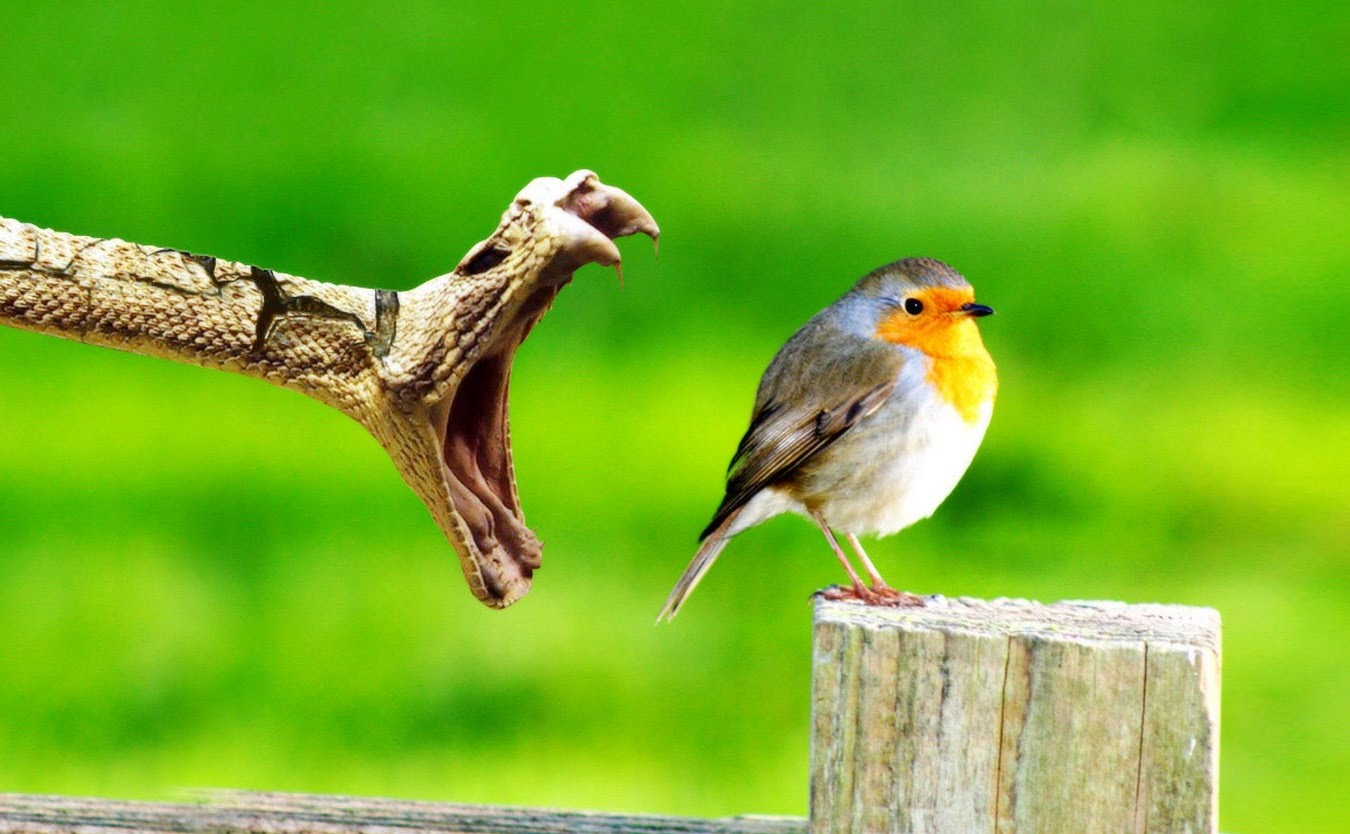
\includegraphics[width=.6\textwidth]{Pictures/Example.jpg}	
	\caption{This is a picture. Source: \citet{isover}}
	\label{Bird}
\end{figure}


\begin{figure} [H]
	\centering
	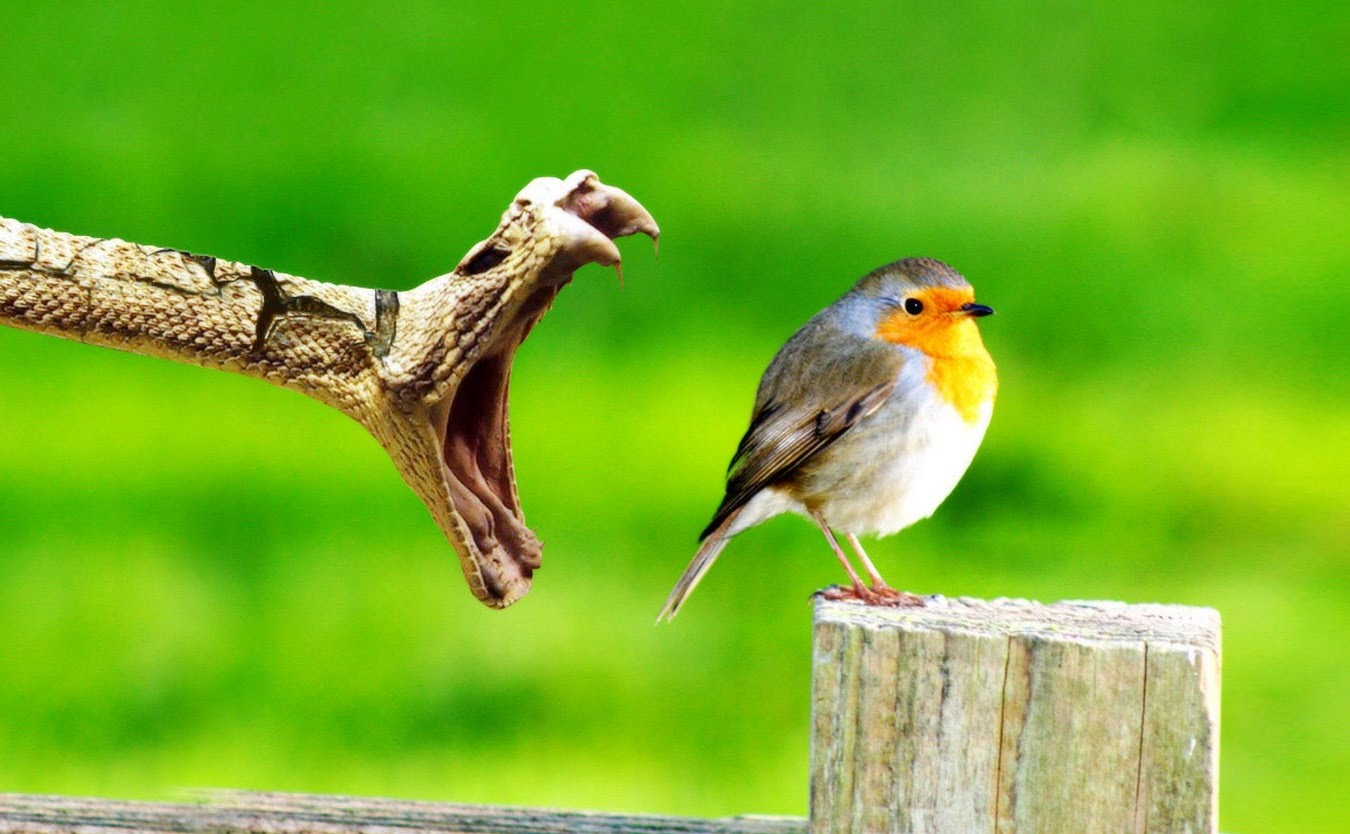
\includegraphics[width=.6\textwidth, angle=-90]{Pictures/Example.jpg}	
	\caption{This picture has been turned}
	\label{BirdTurned}
\end{figure}


\textbf{Cutting a picture}

\begin{figure} [H]
	\centering
	% trim={<left> <lower> <right> <upper>}
    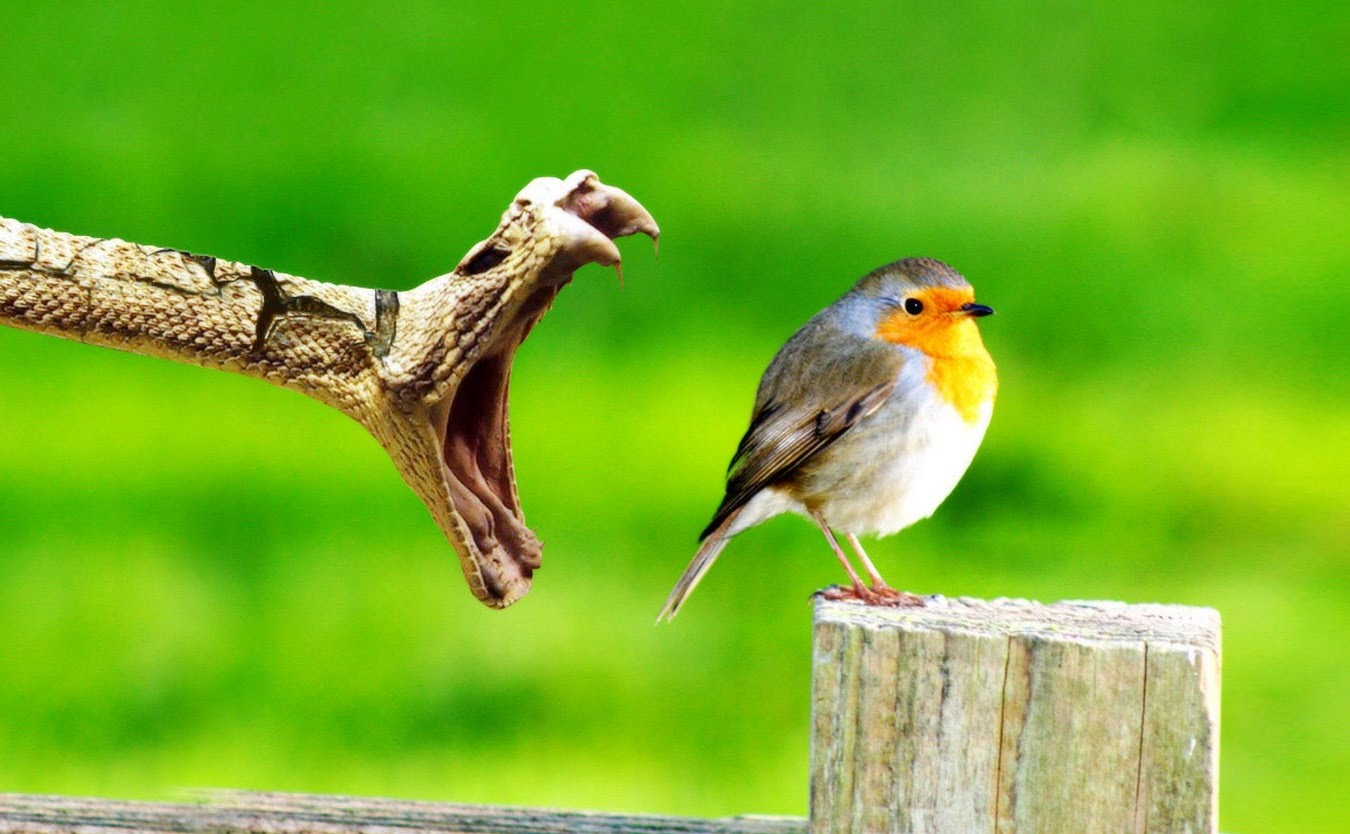
\includegraphics[width=.5\textwidth, trim={23cm 0 0 0},clip]{Pictures/Example.jpg}
	\caption{This picture has been cut}
	\label{BirdCut}
\end{figure}


Referencing to a particular figure is done like this:



\subsection{The Minipage}

\begin{figure} [h]
\begin{minipage}[t]{0.45\textwidth}
\centering
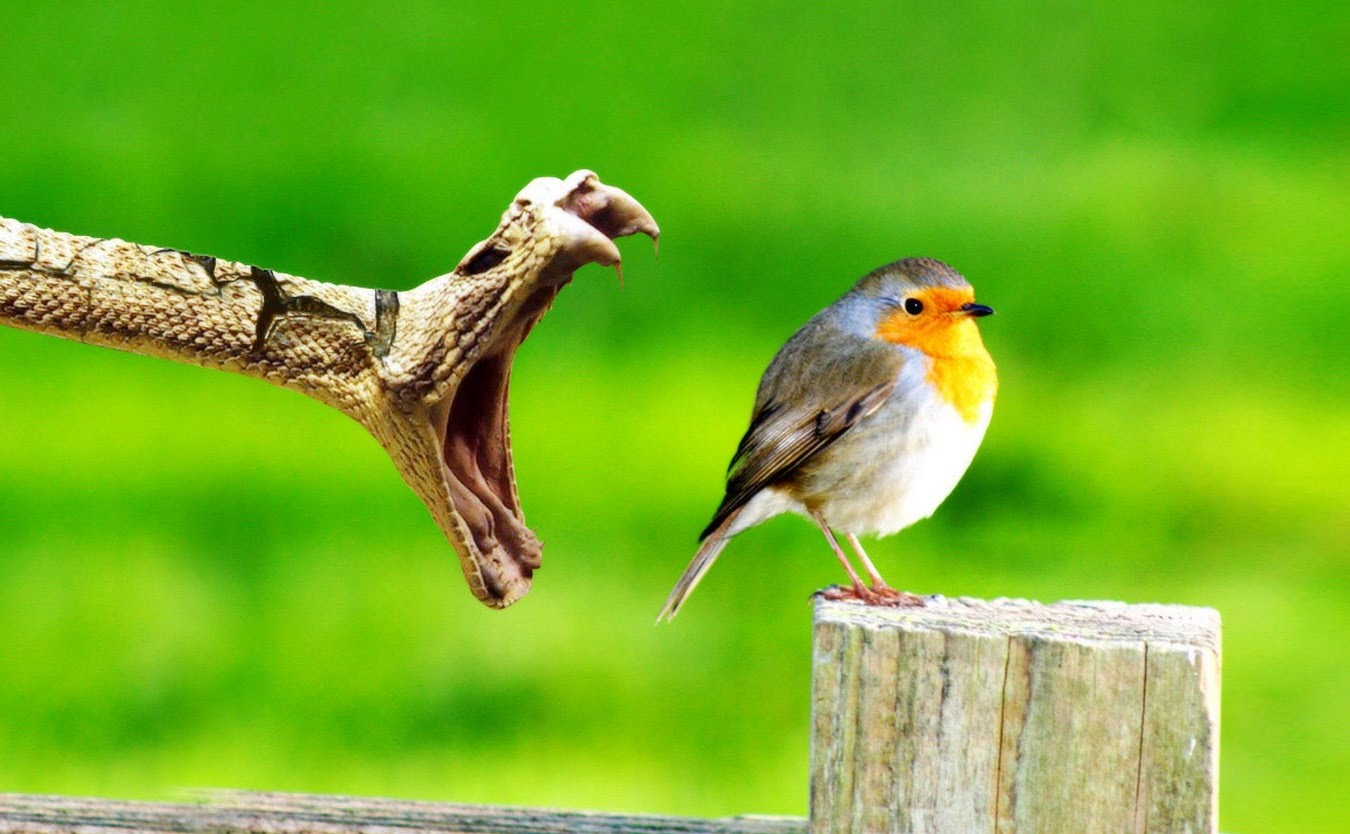
\includegraphics[width=1\textwidth]{Pictures/Example.jpg}
\caption{There is the same picture again}
\label{Bird2}
\end{minipage}
\hspace{0.1\textwidth}
\begin{minipage}[t]{0.45\textwidth}
\centering
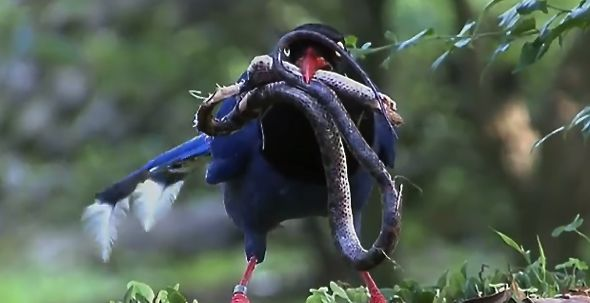
\includegraphics[width=1\textwidth]{Pictures/Example2.jpg}
\caption{Here is another picture.}
\label{Bird3}
\end{minipage}
\end{figure}

Sizes can be adjusted using this part: %\begin{minipage}[t]{0.3\textwidth}

\begin{figure} [h]
\begin{minipage}[t]{0.6\textwidth}
\centering
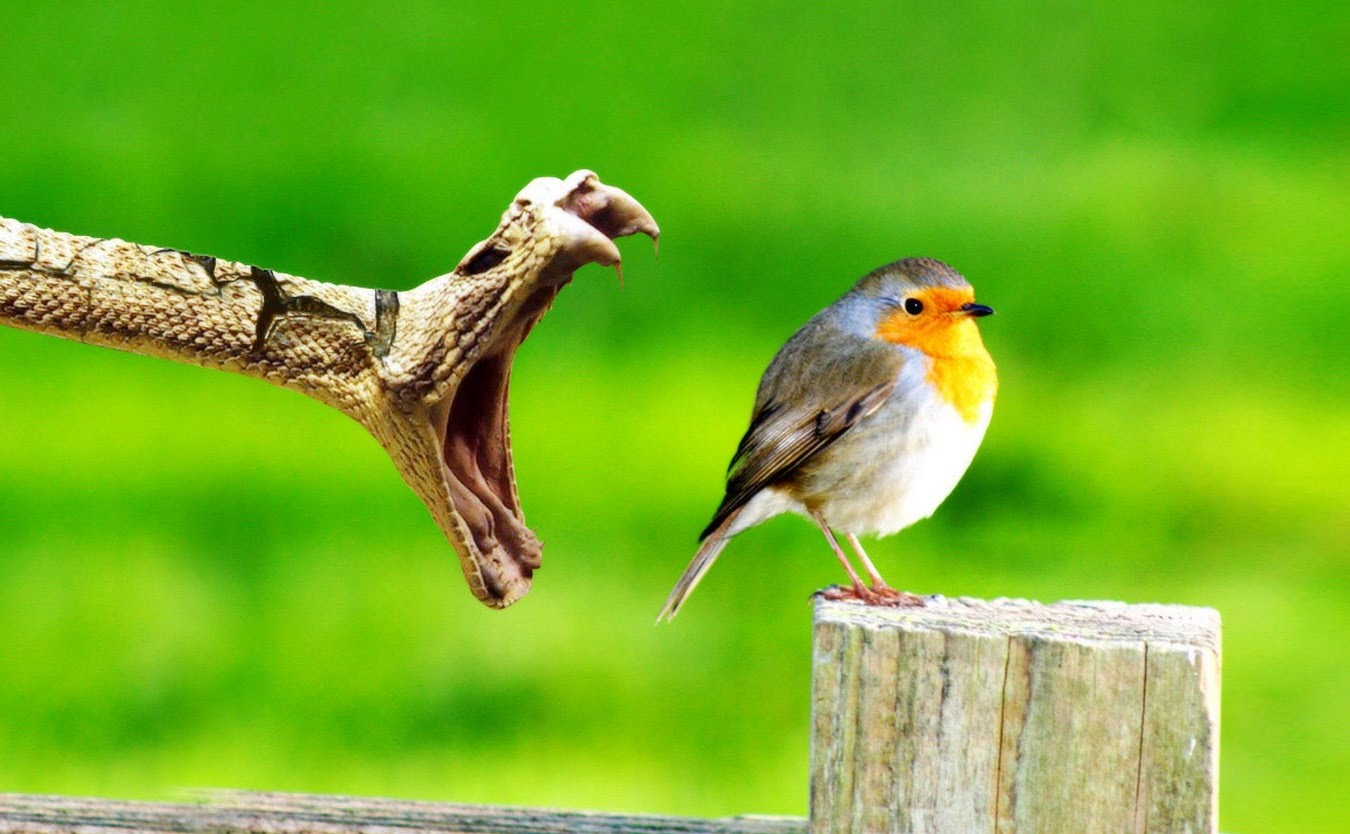
\includegraphics[width=1\textwidth]{Pictures/Example.jpg}
\caption{There is the same picture again}
\label{Bird4}
\end{minipage}
\hspace{0.05\textwidth}
\begin{minipage}[t]{0.3\textwidth}
\centering
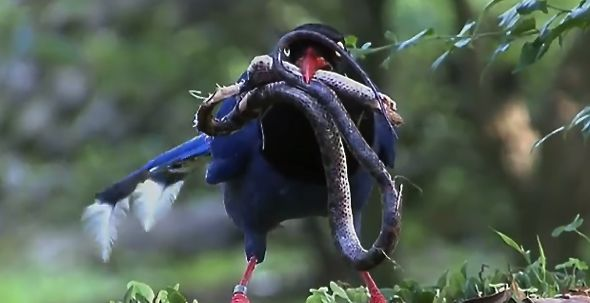
\includegraphics[width=1\textwidth]{Pictures/Example2.jpg}
\caption{Here is another picture. Source: \citet{isover}}
\label{Bird5}
\end{minipage}
\end{figure}







Making references to pictures are done by 